\newpage
ҒТАМР 06.52.17
\hfill {\bfseries \href{https://doi.org/10.58805/kazutb.v.3.24-519}{https://doi.org/10.58805/kazutb.v.3.24-519}}

\sectionwithauthors{С.Рейдолда, О.А. Карпенко, К.Ж. Садвокасова, А.М. Бержанова, Б.Н. Жабытай, А.К. Алпысбаева}{МЕМЛЕКЕТТІК-ЖЕКЕ МЕНШІК ӘРІПТЕСТІКТІҢ АҚМОЛА ӨҢІРІНІҢ
ЭКОНОМИКАЛЫҚ ӨСУІНЕ ӘСЕРІН ТАЛДАУ}

\begin{center}
{\bfseries \textsuperscript{1}С.Рейдолда\envelope, \textsuperscript{2}О.А. Карпенко, \textsuperscript{1}К.Ж. Садвокасова, \textsuperscript{3}А.М. Бержанова, \textsuperscript{1}Б.Н. Жабытай\envelope, \textsuperscript{1}А.К. Алпысбаева}

\textsuperscript{1}Қазақ технология және бизнес университеті, Астана,
Қазақстан,

\textsuperscript{2}РУДН, Мәскеу, Ресей,

\textsuperscript{3}Л.Н. Гумилев атындағы Еуразия ұлттық университеті,
Астана, Қазақстан
\end{center}
\envelope Корреспондент-автор: Saulegul0408@gmail.com, bayana\_7778@mail.ru

Мақаланың мақсаты Ақмола өңірінің экономикалық өсуіне МЖӘ әсерін анықтау
болып табылады. Зерттеу объектісі Ақмола облысында жүзеге асырылған МЖӘ
жобалары және өңірдің әлеуметтік-экономикалық даму процесі. Талдау
нәтижесі бойынша өңірдің экономикалық өсуіне МЖӘ әсері бағаланды.
Зерттеу барысында Ақмола өңірі бойынша жүзеге асырылған МЖӘ жобаларына
динамикалық талдау жасалды. Талдау барысында 2018-2022 жылдар аралығында
МЖӘ жобалары және өңірдің экономикалық өсуін сипаттайтын экономикалық
көрсеткіштер туралы ақпараттар қолданылды. Хоррард-Домер моделін қолдана
отырып, өңірдің экономикалық өсуі анықталды және оған әсер еткен
факторларға факторлық талдау жасалды. Ақмола облысында 2018-2022 жылдар
аралығында барлығы 66 МЖӘ жобасы жүзеге асырыла бастаған, барлығы
7783,26 мың теңге көлемінде инвестиция тартты және осы жылдар аралығында
тартылған инвестициялар орташа есеппен 15,36\% үлесті құрады. Р. Харрод
пен Е. Домар моделі бойынша экономиканың өсу қарқыны мынаны көрсетті:
инвестицияның жиынтық табысқа қатынасы орташа есеппен 0,88 млн тг,
капитал сыйымдылығы 2,25 млн тг, экономиканың өсу қарқыны 0,38 немесе
38,26\% өскен. Қорыта келгенде, Ақмола облысы бойынша МЖӘ сәтті жүзеге
асыру үшін тұрақты инвестициялық климат құру қажет.

{\bfseries Түйін сөздер.} Мемлекеттік-жекеменшік әріптестік, жобалары,
инвестициялар, салыстырмалы талдау, динамикалық талдау, құрылымдық
талдау.

\sectionheading{АНАЛИЗ ВЛИЯНИЯ ГОСУДАРСТВЕННО-ЧАСТНОГО ПАРТНЕРСТВА НА
ЭКОНОМИЧЕСКИЙ РОСТ АКМОЛИНСКОГО РЕГИОНА}

\begin{center}
{\bfseries \textsuperscript{1}С.Рейдолда\envelope,
\textsuperscript{2}О.А. Карпенко, \textsuperscript{1}К.Ж. Садвокасова,
\textsuperscript{3}А.М. Бержанова,}

{\bfseries \textsuperscript{1}Б.Н. Жабытай\envelope,
\textsuperscript{1}А.К. Алпысбаева}

\textsuperscript{1}Казахский университет технологии и бизнеса, Астана,
Казахстан,

\textsuperscript{2} РУДН, Москва, Россия,

\textsuperscript{3} Евразийский национальный университет имени Л.Н.
Гумилева,

e-mail: Saulegul0408@gmail.com, bayana\_7778@mail.ru
\end{center}

Целью статьи является определение влияния ГЧП на экономический рост
Акмолинской области. Объектом исследования являются проекты ГЧП,
реализуемые в Акмолинской области, и процесс социально-экономического
развития региона. По результатам анализа проведена оценка влияния ГЧП на
экономический рост региона. В ходе исследования был проведен
динамический анализ проектов ГЧП, реализуемых в Акмолинской области. В
анализе использовалась информация о проектах ГЧП на 2018-2022 годы и
экономические показатели, характеризующие экономический рост региона. С
помощью модели Хоррарда-Домера был определен экономический рост региона
и проведен факторный анализ факторов, влияющих на него. В Акмолинской
области в период с 2018 по 2022 год всего было реализовано 66 проектов
ГЧП с привлечением инвестиций на сумму 7783,26 тыс. тенге, а
привлеченные инвестиции за годы составили в среднем 15,36\%. Темп роста
экономики по модели Р. Харрода и Е. Домара показал следующее: отношение
инвестиций к общему доходу в среднем составило 0,88 млн. тенге,
капиталоемкость составила 2,25 млн. тенге, темп роста экономики
увеличился на 0,38 или 38,26\%. Для успешной реализации ГЧП в
Акмолинской области необходимо создать стабильный инвестиционный климат.

{\bfseries Ключевые слова.} Государственно-частное партнерство, проекты,
инвестиции, сравнительный анализ, динамический анализ

\sectionheading{ANALYSING THE IMPACT OF PUBLIC-PRIVATE PARTNERSHIP ON THE
ECONOMIC GROWTH OF THE AKMOLA REGION}

\begin{center}
{\bfseries \textsuperscript{1}S. Reidolda\envelope,
\textsuperscript{2} O.A. Karpenko, \textsuperscript{1}K.Zh.
Sadvokassova, \textsuperscript{3}A.M. Berzhanova,}

{\bfseries \textsuperscript{1}B.N. Zhabytai\envelope,
\textsuperscript{1}А.К.} {\bfseries Аlpysbayeva}

\textsuperscript{1}Kazakh University of Technology and Business, Astana,
Kazakhstan,

\textsuperscript{2}RUDN, Moscow, Russia,

\textsuperscript{3}L.N. Gumilev Eurasian National university, Astana,
Kazakhstan,

e-mail: Saulegul0408@gmail.com, bayana\_7778@mail.ru
\end{center}

The purpose of the article is to determine the impact of PPP on the
economic growth of Akmola region. The object of the study is PPP
projects implemented in Akmola region and the process of socio-economic
development of the region. According to the results of the analysis, the
impact of PPP on the economic growth of the region was assessed. In the
course of the study a dynamic analysis of PPP projects implemented in
Akmola region was carried out. The analysis used information on PPP
projects for 2018-2022 and economic indicators characterizing the
economic growth of the region. Using the Horrard-Domer model, the
economic growth of the region was determined and a factor analysis of
the factors affecting it was conducted. In Akmola region in the period
from 2018 to 2022, a total of 66 PPP projects were implemented with the
attraction of investments in the amount of 7783.26 thousand tenge, and
the attracted investments for the years amounted to an average of
15.36\%. The growth rate of the economy according to the model of R.
Harrod and E. Domar showed the following: the ratio of investment to
total income averaged 0.88 million tenge, capital intensity amounted to
2.25 million tenge, the growth rate of the economy increased by 0.38 or
38.26\%. For successful implementation of PPP in Akmola region it is
necessary to create a stable investment climate.

{\bfseries Keywords.} Public-private partnership, projects, investments,
comparative analysis, dynamic analysis.

\begin{multicols}{2}
{\bfseries Кіріспе.} Төмен сапалы инфрақұрылым елдің тұрақты экономикалық
өсуіне және халықаралық нарықта бәсеке қабілеттілігін арттыруға кедергі
келтіреді. Дамымаған инфрақұрылым халықтың өмір сүру сапасының төмен
болуының негізгі себептерінің бірі болып табылады. Сондықтан
инфрақұрылымдық жобалардың әлеуметтік тиімділігі елеулі болады.
Инфрақұрылымға салынатын инвестицияның өсуі халықтың әл-ауқатының
жақсаруына ықпал етеді. Алайда мемлекеттік сектор инфрақұрылымдық
қызметтерді бюджеттен қаржыландырады. Осыған қарамастан инвестицияны
тартудың тиімді жолдарын үнемі іздестіреді. МЖӘ инфрақұрылымға
инвестиция тартудың маңызды құралы болып табылады. Бұл жерде МЖӘ
инфрақұрылымдық қызметті кеңейту және жақсарту мақсатында мемлекет пен
жеке сектор арасында жасалатын келісім-шарт ретінде кең мағынада
қарастырылады {[}1{]}.~

Көп жағдайда МЖӘ тетігін қолданатын жобалар жеткілікті қаржыландырулар
мен эксперттердің көмегінсіз асығыс жасалады. Бұл үлкен қателік. Негізі
МЖӘ жобалары салалық стратегиялармен экономикалық саясаттың бөлігі болып
табылатын басым бағыттағы стратегиялық жобалар болуы тиіс. Мемлекеттің
негізгі рөлі жобаны тиісті деңгейде жүзеге асыруды қамтамасыз ету, жеке
инвесторлардың қызметін қадағалау, туындаған даулы мәселелерді жедел
шешу болып табылады. МЖӘ тетігін қолдану шығыны көп және ұзақ уақытқа
созылуы мүмкін {[}2{]}. Тіпті МЖӘ дамыған елдердің өзінде жобаларды
дайындауға орташа есеппен барлық жұмсалатын шығынның 2,6\% тиесілі және
дайындық кезеңінің ұзақтығы 36 айға созылады. Осыған байланысты қандайда
бір инфрақұрылымға байланысты мәселелерді шешу үшін МЖӘ тетігін қолдану
қаншалық тиімді деген сұрақ туындайды. Алайда мемлекет МЖӘ тетігін
қолдануды қажет етуінің бірқатар себептері бар:

\begin{itemize}
\item
  мемлекеттік сатып алу әдістерінде коррупцияның болуы, жеке
  секторлардың қаржыландыру жолдарының ашық еместігі және қызметінің
  тиімділігінің төмендігі;
\item
  басқарушы және техникалық мамандардың жеткіліксіздігі;
\item
  инфрақұрылымдық жобаларды жүзеге асыру шығындарының көп болуы, кезең
  сайын жөндеу және қамтамасыз ету шығындарының елеулілігі, мемлекеттік
  ресурстардың жетіспеушілігі мен инвестицияға деген қажеттіліктің
  болуы.
\end{itemize}

МЖӘ тетігін қолдану мемлекетке бірқатар пайда әкеледі. Осыған байланысты
МЖӘ жобалары Қазақстан Республикасында 2006 жылдан бастап іске
асырылуда. Соңғы уақытта МЖӘ жандануы заңнамалық және институционалдық
базаны жетілдірумен байланысты болды. 2012 жылдан бастап 2020 жылға
дейінгі кезеңде заңнамаға МЖӘ саласын кеңейтуге бағытталған өзгерістер
енгізілді және МЖӘ жобаларын қарау кезінде жергілікті атқарушы
органдардың дербестігі кеңейтілді. МЖӘ туралы Заңға сәйкес мынадай
мүмкіндіктер ұсынылды: МЖӘ экономиканың барлық салаларында пайдалану;
келісім-шарттардың нысандары мен түрлерін кеңейту; жобаға мемлекеттік
мекеме емес, жеке сектор бастамашы болған кезде жеке қаржылық бастаманы
енгізу; МЖӘ жобаларын жоспарлаудың мерзімдерін қысқарту және арнайы
рәсімін әзірлеу {[}3{]}. Бұл мүмкіндіктер МЖӘ келісім-шарттары санының
артуына алып келді. 2023 жылғы жағдай бойынша республикада 2022 жылға
дейінгі кезеңде жалпы алғанда 1313 жоба ұсынылды, оның ішінде 78 жоба
Ақмола облысында жүзеге асырыла бастады және үлесі 5,94\% құрайды
{[}4{]} МЖӘ жобалары санының күрт өсуі оларға талдау жасауды қажет
етеді.

Зерттеу мақсаты -- Ақмола өңірінде жүзеге асырылған МЖӘ жобаларына
динамикалық, корреляциялық-регрессиялық талдау жасай отырып, МЖӘ өңірдің
экономикалық өсуіне әсерін анықтау. Қойылған мақсатқа сәйкес келесі
міндеттер қойылды:

- Ақмола облысында 2018-2022 жылдар аралығында жасалған МЖӘ
келісім-шарттары бойынша ұсынылған және жүзеге асырылған жобаларға
динамикалық талдау жасау;

- жүзеге асырылған МЖӘ жобаларына құрылымдық және
корреляциялық-регрессиялық талдау жасау;

- өңірдің экономикалық өсуіне МЖӘ жобалардың әсерін анықтау.

{\bfseries Материалдар және әдістер.} Зерттеу нысаны Ақмола облысындағы
2018-2022 жылдардағы МЖӘ жобаларының саны болып табылады. Зерттеу пәні
өңірдің МЖӘ жобаларына талдау жасау.

Мемлекеттік-жекеменшік әріптестік - бұл 1990 жылдардың басында Еуропада
мемлекеттің нарықтық экономикаға қатысуының жаңа құралы және
жекешелендіруге балама ретінде пайда болған жаңа институт {[}5{]}.
Шетелдік МЖӘ зерттеулерінің ішінде Хакман, Р.Дж. Беннетт пен Г. Кребс
1994, Дж. Селлгрена (1990), Э.Осборна (2003), С. Стерн және Д. Хардина
(2005), Дж. Бродбент және Дж. Левфлина 2003, Ходж және К.Грива (2007),
Э.Р. Яскомба (2007) және т. б. атап өтуге болады.~

МЖӘ шетелдік зерттеулер шеңберінде бірнеше тұжырымдамалық тәсілдерді
бөліп көрсетуге болады. МЖӘ экономикадағы өз орны мен рөлін анықтады:

1. МЖӘ сөзі кең мағынада қайырымдылыққа, корпоративтік әлеуметтік
жауапкершілікке және т. б. негізделген бизнес пен мемлекет
ынтымақтастығының кез келген нысаны ретінде түсіндірілді {[}6{]}.

2. МЖӘ ұйымдық құрылым және «жаңа мемлекеттік басқару» құралы ретінде
Ю.Ван Хам және Д. К. Коппен Жан (2001), Дж. Бродбент және Дж. Льюфлин
(2003). жұмыстарында ескерілді. Осы тәсілге сәйкес МЖӘ мемлекеттік
реттеудің, мемлекеттік меншіктің стратегиялық және өмірлік маңызды
объектілерін жекешелендірудің баламасы ретінде түсіндірілді. Алайда, бұл
зерттеулер тиімді ұйымдастырушылық тетіктерді мен әдістерді табуға
бағытталған {[}7{]}.

3. Е.С. Саваз (2000), М. Губельман және Х. Дельмонет (1983) «сөз ойыны»
деп түсіндірді. Мұндай тәсілге сәйкес авторлар жағымды емес, жағымсыз
жақтары мен МЖӘ тәуекелдерін атап өтті. Олар кемшіліктер мен мәселелерді
қоса отырып, мемлекеттік объектілерді жекешелендірудің жасырын нысаны
екенін түсіндірді {[}8{]}.

4. МЖӘ тетігі ұлттық, халықаралық, өңірлік, қалалық, муниципалдық,
экономикалық және әлеуметтік даму құралы ретінде түсіндірілді {[}9{]}.

Мемлекет пен жеке бизнес арасындағы қарым-қатынастың теориялық негіздері
шетелдік экономистер Фишер г., Портер М., Стиглиц Д. және басқалардың
зерттеулерінде көрсетілген. Тұжырымдаманың ТМД және МЖӘ практикасындағы
негіздері отандық экономикаға тән ерекшеліктерді ескере отырып, В.А.
Королев, В.Г. Барнабский, А.В. Клименко, В.А. Кабашкин және т. б.
қарастырды {[}10{]}.

Қазақстандағы МЖӘ байланысты мәселелер А.В. Пиунованың, Ф. Смағұлованың,
Г.Ш. Ишкининаның және т. б. жұмыстарында қаралған, Қазақстанда МЖӘ
мүмкіндіктері зерделенген және толық көлемде пайдаланылмаған, оның
практикасы қолданыстағы заңнама шеңберінде әріптестіктің рұқсат етілген
нысандарын пайдаланудың бірнеше мысалын ғана анықтауға мүмкіндік береді.

Шетелдік ғалымдардың жұмыстарында МЖӘ мәні былай қарастырылған:

\begin{itemize}
\item
  Ходж және К.Грива еңбектеріне сәйкес МЖӘ мемлекеттік және жеке ұйымдар
  арасындағы тығыз ұйымаралық байланыстарды басқару және қаржыландыру
  тетігі ретінде қарау ұсынылады {[}11{]}.
\item
  Ю. Ван Хам және Д. К. Коппен МЖӘ институционалдық тұрғыдан мемлекеттік
  және жеке құрылымдар арасындағы белгілі бір ынтымақтастық, осы
  ынтымақтастық аясында өнімдер мен қызметтер өндірісін бірлесіп дамыту
  және осыған байланысты шығындар мен ресурстарды, тәуекелдерді бөлу деп
  түсіндірді. Басқа тұрғыдан алғанда, МЖӘ «құрылыс-иелену-жеткізу» және
  «өсіру-іске қосу-жеткізу» тетіктері арқылы инфрақұрылымдық жобаларға
  қатысу ретінде түсіндіріледі {[}12{]}.
\item
  C. Линдердің балама көзқарасы бойынша МЖӘ - бұл «сөз ойыны», яғни
  серіктестік туралы бірнеше пайдалы сөздер. Бұл сөз жылы және достық
  сөйлемдерден тұрады {[}13{]}. Осылайша, мемлекеттік органдар мен жеке
  бизнес-құрылымдар арасында жақсы үйлестірілген әріптестік қатынастарды
  орнату арқылы инфрақұрылымдық мәселелерді шешуге болады, бірақ МЖӘ
  іске асыру және оның нәтижесін дәл өлшеу мүмкін емес {[}14{]}. Бұл
  көзқарас МЖӘ сыни көзқарас тұрғысынан қарастырылады. Бұдан басқа, МЖӘ
  көптеген кемшіліктері мен мәселелері бар мемлекеттік мүлікті
  жекешелендірудің түрлендірілген нысаны жоғары тәуекелді көрсетеді.
\item
  2015 жылғы 31 қазанда қабылданған «Мемлекеттік-жекешелік әріптестік
  туралы» Заңға сәйкес МЖӘ мемлекеттік әріптес пен МЖӘ сипаттамаларына
  сәйкес келетін жекеше әріптес арасындағы ынтымақтастық нысаны болып
  табылады.
\end{itemize}

Бүгінгі таңда зерттеу нәтижелері бойынша МЖӘ байланысты бірыңғай жалпы
анықтама жоқ екенін атап өтуге болады. Біздің ойымызша, мемлекеттік -
жекеменшік әріптестік (МЖӘ) - бұл инфрақұрылымдық жобаларда кеңінен
қолданылатын мемлекеттік және жеке секторлар арасындағы ынтымақтастық
туралы ұзақ мерзімді концессиялық келісім. Сонымен қатар осы тақырыпты
зерделеудің терең әзірленген әдіснамасы ұсынылмаған, МЖӘ тетіктеріне
экономикалық талдау жүргізілген жоқ.

Зерттеу барысында экономикалық-статистикалық топтау, динамикалық талдау,
құрылымдық талдау, салыстырмалы талдау әдістері қолданылды. Ақмола
облысында іске асырылған МЖӘ жобаларды топтастыру әдісімен экономика
салалары бойынша топтастырылды. Динамикалық талдау әдісімен 2018 жылдан
бастап 2022 жылға дейінгі кезеңде іске асырылған МЖӘ жобаларының
абсолюттік өсу қарқыны мен өсім қарқыны айқындалды. Р. Харрод пен Е.
Домар моделі бойынша экономиканың өсу қарқынын есептеу үшін келесі
формула қолданылды {[}15{]}:

TP = S / C

мұндағы, ТР -- экономикалық өсу қарқыны;

S - инвестицияның жиынтық табысқа қатынасы;

C - капитал сыйымдылығы.

Экономиканың өсу қарқынына факторлық талдау жасау үшін келесі формулалар
қолданылды:

$\Delta TP_s=\frac{S_1}{C_0}-\frac{S_1}{C_0}$- инвестицияның жиынтық табысқа
қатынасының өзгеру әсерінен экономикалық өсу қарқынының өзгеруі;

$\Delta TP_c=\frac{S_1}{C_1}-\frac{S_1}{C_0}$- капитал сыйымдылығының өзгеру
әсерінен экономикалық өсу қарқынының өзгеруі;

$\Delta TP=\Delta TP_c\pm \Delta TP_s$ - факторлардың өзгеру әсерінен
экономикалық өсу қарқынының жалпы өзгеруі.

{\bfseries Нәтижелер және талқылау.} 2018-2022 жылдар аралығында Ақмола
облысында жүзеге асырылған МЖӘ жобаларының саны туралы ақпараттар
1-суретте келтірілген:
\end{multicols}

\begin{figure}[H]
	\centering
	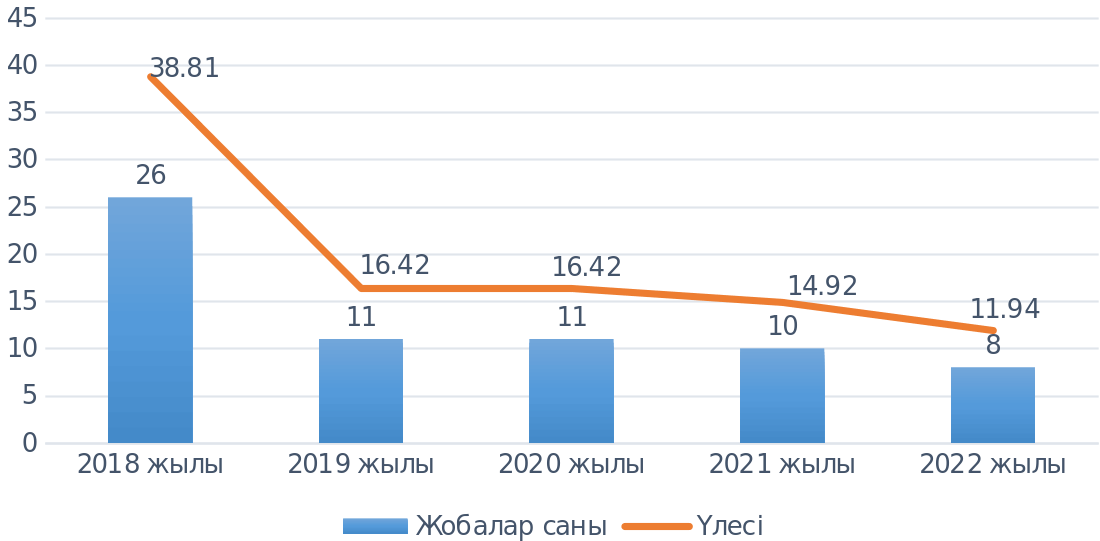
\includegraphics[width=0.7\textwidth]{assets/340.3}
	\caption*{1-сурет. 2018-2022 жылдарғы Ақмола облысы бойынша жүзеге
асырылған МЖӘ жобаларының саны}
	\caption*{\normalfont \emph{Ескерту - {[}4{]} әдебиеттен алынған мәліметтер негізінде
авторлармен құрастырылған}}
\end{figure}

\begin{multicols}{2}
1-суретке сәйкес Ақмола облысында 2018-2022 жылдар аралығында барлығы 66
МЖӘ жобасы жүзеге асырыла бастаған, ең көп жоба 2018 жылға тиесілі және
одан кейінгі жылдары күрт азайғандығын көруге болады. Сонымен жүзеге
асырылған жобалардың үлесі 2018 жылы -- 38,81\%, 2019 жылы -- 16,42\%,
2020 жылы -- 16,42\%, 2021 жылы -- 14,92\%, 2022 жылы - 11,94\% құраған.

МЖӘ жобалары әр түрлі салаларды қамтыған. Ең көбі білім беру саласында
-54 жоба, денсаулық сақтау -- 6 жоба, энергетика және тұрғын үй
коммунальдық шаруашылығы -- 1 жоба, көлік және инфрақұрылым -- 4 жоба,
ауылшаруашылығында -- 1 жоба нақты іске асырылып жатыр. Нақты іске
асырылып жатқан жобалардың экономика салалары бойынша үлесі де анықталды
және салалар бойынша үлесі келесі 2-суретте берілген:
\end{multicols}

\begin{figure}[H]
	\centering
	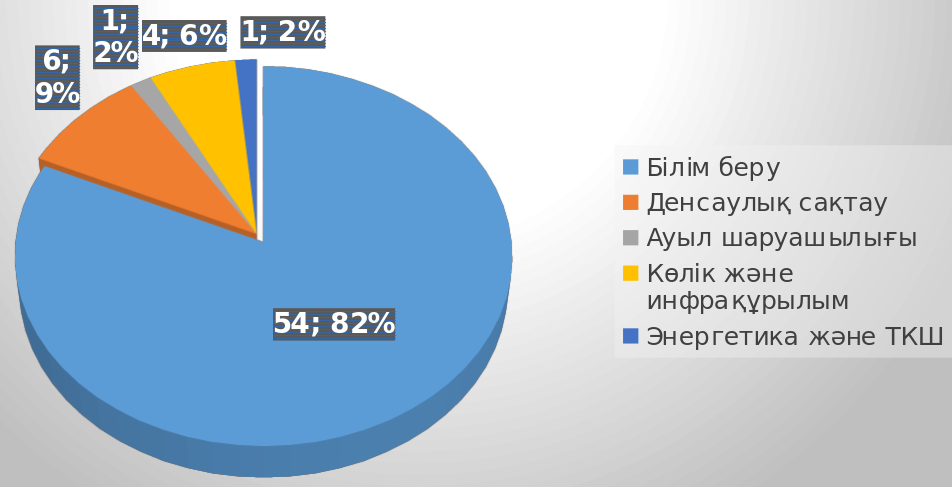
\includegraphics[width=0.5\textwidth]{assets/340.4}
	\caption*{2-сурет. Ақмола облысы бойынша МЖӘ жобаларының құрылымы}
	\caption*{\normalfont \emph{Ескерту - {[}4{]} әдебиеттен алынған мәліметтер негізінде авторлармен құрастырылған}}
\end{figure}

\begin{multicols}{2}
2-суретке сәйкес МЖӘ жобаларының ішінде білім беру саласы бойынша
жасалған жобалардың үлесі - 82\%, денсаулық сақтау саласы - 9\%,
энергетика және тұрғын үй коммунальдық шаруашылығы саласы -- 2\%, көлік
және инфрақұрылым саласы - 6\% және ауыл, орман және балық шаруашылығы
саласы - 1\% құрап отыр. МЖӘ жобалары бойынша ең көп келісім-шарт
жасалған сала білім беру саласы, өйткені республика деңгейінде мектепке
дейінгі білім беру мәселесі өте өзекті болған еді. МЖӘ арқылы
балабақшалар жұмысын тиімді ұйымдастыруға жеке бизнес өкілдері белсенді
араласып, балабақша тапшылығын толықтай жойды.

Әрі қарай Ақмола облысының экономикалық өсу қарқынына талдау жасалды
және нәтижесі келесі 1-кесте берілген.
\end{multicols}

\begin{table}[H]
\caption*{1 - кесте. 2018-2022 жылдарғы Ақмола облысының экономикалық өсу қарқыны}
\centering
\begin{tabular}{|lllllll|}
\hline
\multicolumn{1}{|l|}{Көрсеткіштер} &
  \multicolumn{1}{l|}{2018} &
  \multicolumn{1}{l|}{2019} &
  \multicolumn{1}{l|}{2020} &
  \multicolumn{1}{l|}{2021} &
  \multicolumn{1}{l|}{2022} &
  Орташа өсу қарқыны, \% \\ \hline
\multicolumn{1}{|l|}{ЖӨӨ өсу қарқыны} &
  \multicolumn{1}{l|}{109,5} &
  \multicolumn{1}{l|}{113,7} &
  \multicolumn{1}{l|}{118,1} &
  \multicolumn{1}{l|}{117,3} &
  \multicolumn{1}{l|}{125,3} &
  116,78 \\ \hline
\multicolumn{1}{|l|}{ЖӨӨ өсім қарқыны} &
  \multicolumn{1}{l|}{9,5} &
  \multicolumn{1}{l|}{13,7} &
  \multicolumn{1}{l|}{18,1} &
  \multicolumn{1}{l|}{17,3} &
  \multicolumn{1}{l|}{25,3} &
  16,78 \\ \hline
\multicolumn{1}{|p{0.25\textwidth}|}{Өнеркәсіптік өндіріс көлемінің өсім қарқыны} &
  \multicolumn{1}{l|}{23,2} &
  \multicolumn{1}{l|}{17,5} &
  \multicolumn{1}{l|}{19,9} &
  \multicolumn{1}{l|}{31,5} &
  \multicolumn{1}{l|}{9,5} &
  20,32 \\ \hline
\multicolumn{7}{|l|}{\textit{Ескерту - {[}4{]} әдебиеттен алынған мәліметтер негізінде авторлармен құрастырылған}} \\ \hline
\end{tabular}
\end{table}

\begin{multicols}{2}
1-кестеге сәйкес 2018-2022 жылдары аралығында Ақмола облысының
экономикалық өсу қарқыны орташа есеппен 116,78\%, орташа өсім қарқыны
16,78\% және өнеркәсіптік өндіріс көлемі орташа өсім қарқыны 20,32\%
құраған. ЖӨӨ өсім қарқының құлашы 15,8\% құраған. Ең жоғарғы өсім
қарқыны 2022 жылы 25,3\% құраған және ең төменгі өсім қарқыны 2018 жылы
9,5\% құраған. Өнеркәсіптік өндіріс көлемінің ең жоғарғы өсім қарқыны
2021 жылы - 31,5\% өскен болса, ең төменгі өсім қарқыны 2022 жылы --
9,5\% өскенін көруге болады. Бұл көрсеткіштің 2018-2020 жылдар
аралығында кемігендігін байқауға болады.

Р. Харрод пен Е. Домар моделі бойынша экономиканың өсу қарқынына
талдауға қажетті мәліметтердің орташа абсолюттік өсімі есептелді және
талдау нәтижесі 2-кестеде берілген.
\end{multicols}

\begin{table}[H]
\caption*{2 - кесте. 2018-2022 жылдарғы Ақмола облысының экономикалық өсу
қарқынын сипаттайтын көрсеткіштердің орташа абсолютті өсімі}
\centering
\begin{tabular}{|lllllll|}
\hline
\multicolumn{1}{|l|}{Көрсеткіштер} &
  \multicolumn{1}{l|}{2018} &
  \multicolumn{1}{l|}{2019} &
  \multicolumn{1}{l|}{2020} &
  \multicolumn{1}{l|}{2021} &
  \multicolumn{1}{l|}{2022} &
  Орташа абсолюттік өсім \\ \hline
\multicolumn{1}{|p{0.25\textwidth}|}{Негізгі капитал, млрд тг} &
  \multicolumn{1}{l|}{145,3} &
  \multicolumn{1}{l|}{1619,3} &
  \multicolumn{1}{l|}{1481,5} &
  \multicolumn{1}{l|}{1683,8} &
  \multicolumn{1}{l|}{2162,8} &
  1418,54 \\ \hline
\multicolumn{1}{|p{0.25\textwidth}|}{Өндірілген өнімнің көлемі, млрд тг} &
  \multicolumn{1}{l|}{536,4} &
  \multicolumn{1}{l|}{553,3} &
  \multicolumn{1}{l|}{686,4} &
  \multicolumn{1}{l|}{827} &
  \multicolumn{1}{l|}{1 542, 2} &
  650,78 \\ \hline
\multicolumn{1}{|p{0.25\textwidth}|}{Жиынтық табыс, млрд тг} &
  \multicolumn{1}{l|}{230,4} &
  \multicolumn{1}{l|}{332} &
  \multicolumn{1}{l|}{516,3} &
  \multicolumn{1}{l|}{484,7} &
  \multicolumn{1}{l|}{1 936,6} &
  390,85 \\ \hline
\multicolumn{1}{|p{0.25\textwidth}|}{Негізгі капиталға жасалған инвестициялар, млрд тг} &
  \multicolumn{1}{l|}{278,1} &
  \multicolumn{1}{l|}{333,7} &
  \multicolumn{1}{l|}{436,6} &
  \multicolumn{1}{l|}{514, 6} &
  \multicolumn{1}{l|}{566,5} &
  403,73 \\ \hline
\multicolumn{7}{|l|}{\textit{Ескерту - {[}4{]} әдебиеттен алынған мәліметтер негізінде авторлармен құрастырылған}} \\ \hline
\end{tabular}
\end{table}

\begin{table}[H]
\caption*{3 - кесте. 2018-2022 жылдарғы Ақмола облысының экономиканың өсу
қарқынын Р. Харрод пен Е. Домар моделі бойынша талдау}
\centering
\begin{tabular}{|lllllll|}
\hline
\multicolumn{1}{|l|}{Көрсеткіштер} &
  \multicolumn{1}{l|}{2018} &
  \multicolumn{1}{l|}{2019} &
  \multicolumn{1}{l|}{2020} &
  \multicolumn{1}{l|}{2021} &
  \multicolumn{1}{l|}{2022} &
  Орташа өсу қарқыны \\ \hline
\multicolumn{1}{|p{0.25\textwidth}|}{Инвестицияның жиынтық табысқа қатынасы, S} &
  \multicolumn{1}{l|}{1,21} &
  \multicolumn{1}{l|}{1,01} &
  \multicolumn{1}{l|}{0,85} &
  \multicolumn{1}{l|}{1,06} &
  \multicolumn{1}{l|}{0,29} &
  0,88 \\ \hline
\multicolumn{1}{|p{0.25\textwidth}|}{Капитал сыйымдылығы, C} &
  \multicolumn{1}{l|}{2,71} &
  \multicolumn{1}{l|}{2,93} &
  \multicolumn{1}{l|}{2,16} &
  \multicolumn{1}{l|}{2,04} &
  \multicolumn{1}{l|}{1,4} &
  2,25 \\ \hline
\multicolumn{1}{|p{0.25\textwidth}|}{Экономиканың өсу қарқыны, ТР} &
  \multicolumn{1}{l|}{0,45} &
  \multicolumn{1}{l|}{0,34} &
  \multicolumn{1}{l|}{0,39} &
  \multicolumn{1}{l|}{0,52} &
  \multicolumn{1}{l|}{0,21} &
  0,38 \\ \hline
\multicolumn{1}{|p{0.25\textwidth}|}{Экономиканың өсу қарқыны, ТР, \%} &
  \multicolumn{1}{l|}{44,6} &
  \multicolumn{1}{l|}{34,4} &
  \multicolumn{1}{l|}{39,2} &
  \multicolumn{1}{l|}{52,2} &
  \multicolumn{1}{l|}{20,9} &
  38,26 \\ \hline
\multicolumn{7}{|l|}{\textit{Ескерту - {[}4{]} әдебиеттен алынған мәліметтер негізінде авторлармен құрастырылған}} \\ \hline
\end{tabular}
\end{table}

\begin{table}[H]
\caption*{4 - кесте. 2018-2022 жылдарғы Ақмола облысының экономиканың өсу
қарқынын Р. Харрод пен Е. Домар моделі бойынша факторлық талдау}
\centering
\begin{tabular}{|lllllll|}
\hline
\multicolumn{1}{|l|}{Факторлар} &
  \multicolumn{1}{l|}{2018} &
  \multicolumn{1}{l|}{2019} &
  \multicolumn{1}{l|}{2020} &
  \multicolumn{1}{l|}{2021} &
  \multicolumn{1}{l|}{2022} &
  Орташа мәні \\ \hline
\multicolumn{1}{|l|}{1 фактор} &
  \multicolumn{1}{l|}{-0,075} &
  \multicolumn{1}{l|}{-0,075} &
  \multicolumn{1}{l|}{-0,054} &
  \multicolumn{1}{l|}{0,1} &
  \multicolumn{1}{l|}{-0,378} &
  -0,096 \\ \hline
\multicolumn{1}{|l|}{2 фактор} &
  \multicolumn{1}{l|}{0,018} &
  \multicolumn{1}{l|}{-0,028} &
  \multicolumn{1}{l|}{0,103} &
  \multicolumn{1}{l|}{0,03} &
  \multicolumn{1}{l|}{0,065} &
  0,038 \\ \hline
\multicolumn{1}{|l|}{Жалпы өзгерісі} &
  \multicolumn{1}{l|}{0,093} &
  \multicolumn{1}{l|}{-0,102} &
  \multicolumn{1}{l|}{0,048} &
  \multicolumn{1}{l|}{0,13} &
  \multicolumn{1}{l|}{-0,313} &
  -0,029 \\ \hline
\multicolumn{7}{|l|}{\textit{Ескерту - {[}4{]} әдебиеттен алынған мәліметтер негізінде авторлармен құрастырылған}} \\ \hline
\end{tabular}
\end{table}

\begin{multicols}{2}
2-кесте бойынша 2018-2022 жылдар аралығында Ақмола облысы бойынша
экономикалық өсу қарқынын сипаттайтын көрсеткіштердің орташа абсолюттік
өсімі мынаны көрсетті: негізгі капитал -- 1418,54 млрд тг, өндірілген
өнімнің көлемі -- 650,78 млрд тг, жиынтық табыс -- 390,85 млрд тг,
негізгі капиталға жасалған инвестициялар -- 403,73 млрд тг өскен.

Осы көрсеткіштер бойынша Р. Харрод пен Е. Домар моделі негізінде
2018-2022 жылдар аралығында Ақмола облысының экономикалық өсу қарқынына
талдау жасалды және талдау нәтижесі келесі 3-кестеде көрсетілген.

3-кестеге сәйкес 2018-2022 жылдарғы Ақмола облысының экономиканың өсу
қарқынын Р. Харрод пен Е. Домар моделі бойынша мынаны көрсетті:
инвестицияның жиынтық табысқа қатынасы орташа есеппен 0,88 млн тг,
капитал сыйымдылығы 2,25 млн тг, экономиканың өсу қарқыны 0,38 немесе
38,26\% өскен.

Бұдан әрі экономикалық өсуді сипаттайтын көрсеткіштерге факторлық талдау
жасалды және нәтижесі келесі 4-кестеде берілген:

4-кесте бойынша 2018-2022 жылдар аралығында Ақмола облысының
экономикалық өсуі факторлардың өзгеру әсерінен орташа есеппен -0,096 млн
тг азайған, соның ішінде инвестицияның жиынтық табысқа қатынасының азаюы
әсерінен 0,038 млн тг және капитал сыйымдылығының азаюы әсерінен 0,029
млн тг азайған.

Өңірлік экономиканың негізгі және дәстүрлі әдістерінің бірі - өңірлердің
әлеуметтік-экономикалық дамуын талдау. Талдаудың мақсаты -
әлеуметтік-экономикалық даму стратегиясында қарастырылған экономикалық
өсуді негіздеу үшін сәйкессіздіктер мен пайдаланылмаған мүмкіндіктерді
анықтау болып табылады. Осы тұрғыда біздің зерттеу Ақмола облысының
экономикалық дамуына МЖӘ әсерін анықтау болып табылады. Экономикалық
дамуды сипаттау үшін экономикалық өсу коэффициенті қолданылды. 2018-2022
жылдар аралығында Ақмола облысының экономикалық өсуі келесі 4-суретте
көрсетілген:
\end{multicols}

\begin{figure}[H]
	\centering
	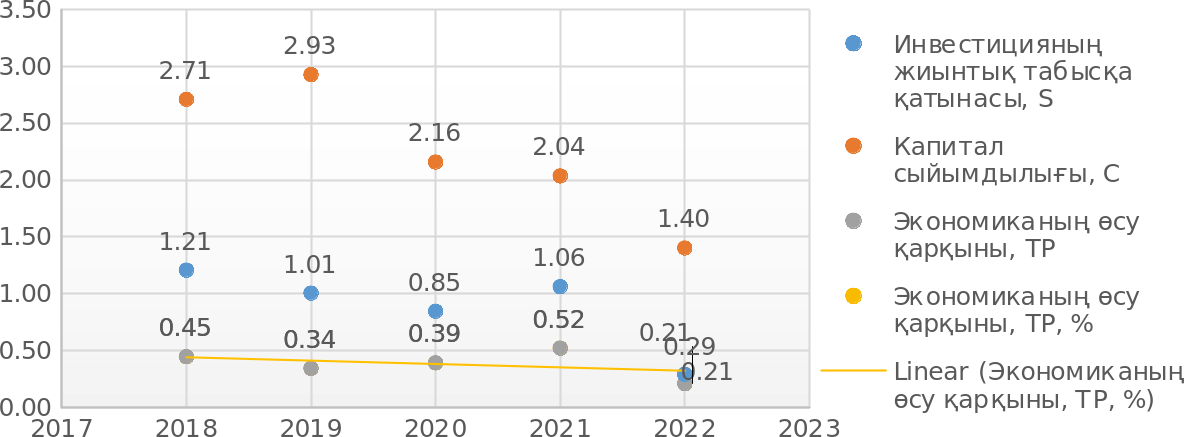
\includegraphics[width=0.8\textwidth]{assets/340.5}
	\caption*{3 - сурет. 2018-2022 жылдары Ақмола облысының экономикалық өсуі}
	\caption*{\normalfont \emph{Ескерту - {[}4{]} әдебиеттен алынған мәліметтер негізінде авторлармен құрастырылған}}
\end{figure}

\begin{figure}[H]
	\centering
	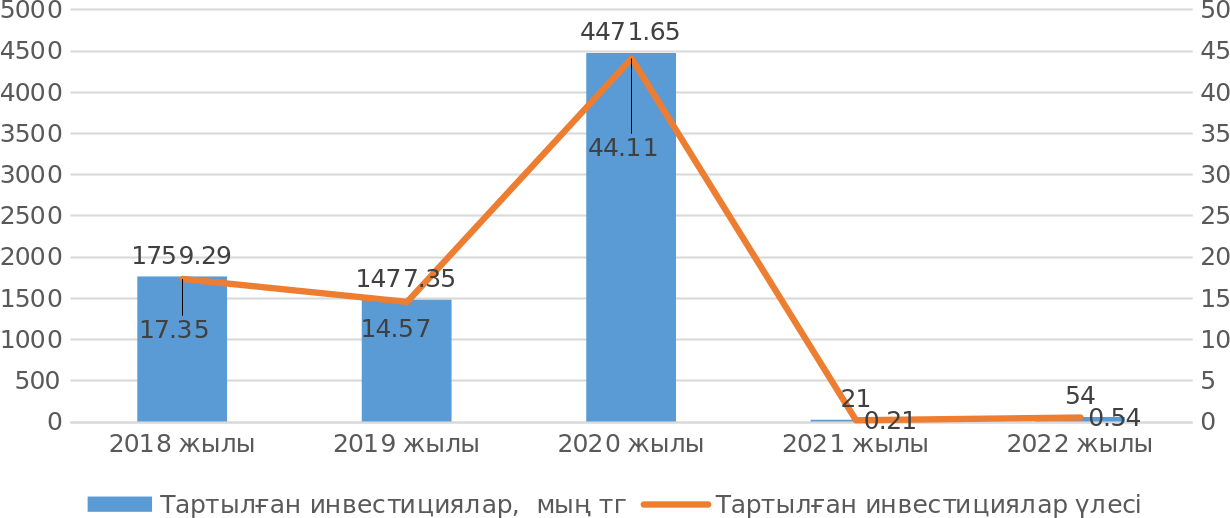
\includegraphics[width=0.8\textwidth]{assets/340.6}
	\caption*{4 - сурет. 2018-2022 жылдарғы Ақмола облысы бойынша жүзеге
асырылған МЖӘ жобаларынан тартылған инвестиция көлемі мен үлесі}
    \caption*{\normalfont \emph{Ескерту - {[}4{]} әдебиеттен алынған мәліметтер негізінде авторлармен құрастырылған}}
\end{figure}

\begin{multicols}{2}
3-суретке сәйкес 2018-2022 жылдары Ақмола облысының экономикалық өсуі
0,45-0,21\% аралығын көрсетеді және жылдан жылға біртіндеп азайған.
Сондай-ақ инвестицияның жиынтық табысқа қатынасы 2,71-1,4 млн тг,
капитал сыйымдылығы 1,21-0,21 млн тг азайған.

2018-2022 жылдар аралығында Ақмола облысы бойынша жүзеге асырылған МЖӘ
жобаларынан тартылған инвестиция көлемі мен оның үлесі туралы келесі
3-суретте берілген:

4-суретке сәйкес Ақмола облысында 2018-2022 жылдар аралығында барлығы
7783,26 мың теңге көлемінде инвестиция тартты және осы жылдар аралығында
тартылған инвестициялар орташа есеппен 15,36\% үлесті құрады. МЖӘ
жобаларынан тартылған инвестиция 2020 жылдан кейін күрт азайып
кеткендігін көреміз, себебі короновирустан кейінгі жағдай қаржылық
тапшылыққа алып келгені бір жағынан, 2020 жылға дейін қаржылық жабылуға
қол жеткізген жобалардың болуы екінші жағынан әсер етті. Сонымен
жобалардан тартылған инвестициялар көлемі мен үлесі 2018 жылы -- 1759,29
мың тг немесе 17,35\%, 2019 жылы -- 1477,35 мың теңге немесе 16,42\%,
2020 жылы -- 4471,65 мың теңге немесе 44,11\%, 2021 жылы -- 21 мың теңге
немесе 0,21\%, 2022 жылы -- 54 мың теңге немесе 0,54\% құраған.

Жалпы Ақмола облысының экономикалық даму деңгейі 2020 жылдан кейін күрт
төмендеген және сәйкесінше МЖӘ тартылған инвестиция да, жалпы
инвестицияда азайғанын көреміз. Оның негізгі себебі короновирус
кезеңінен кейінгі экономикалық құлдырау екендігімен түсіндіруге болады.

{\bfseries Қорытынды.} МЖӘ жобалары өңірдің экономикасын
диверсификациялауға және өсуіне ықпал етеді. Жаңа жобалар, әсіресе
инфрақұрылымдық жобалар, бизнесті дамытуға және экономикалық
белсенділікті арттыруға мүмкіндік береді. Өңірдің
әлеуметтік-экономикалық дамуын қамтамасыз ету үшін МЖӘ арқылы әлеуметтік
маңызы бар жобаларды іске асыруға болады. Ақмола облысында МЖӘ жобаларын
2018 жылдан бастап сәтті жүзеге асыруда. Соңғы жылдары іске асырылған
МЖӘ жобалары туралы сандық ақпаратты экономикалық-статистикалық
талдаумен бағалау, атап айтқанда, экономиканың қандай секторларында
жобалар іске асырылатынын, МЖӘ қандай түрін шаруашылық жүргізуші
субъектілер жиі пайдаланатынын, ұлттық деңгеймен салыстырғанда қанша
инвестиция тартылғанын бағалау және нәтижелерді талқылау орындалды.
Талдау нәтижесі бойынша мынандай қорытынды жасауға болады:

1. Ақмола облысы бойынша барлығы 78 жоба ұсынылған, оның 66 нақты жүзеге
асырыла бастаған, яғни әзірленген жобалардың 68,4\% жүзеге асырылды
дегенді білдіреді. Бұл Ақмола өңірі бойынша МЖӘ жобаларын әзірлеу және
жүзеге асыру белсенділігін көрсетеді.

2. Жобаларды жүзеге асырудың динамикасына жүргізілген талдау бойынша 2018
жылы жүзеге асырылған жобалардың абсолюттік өсімі 21 жобаға немесе 3.5
есеге өскенін байқауға болады. 2018 жылы жобалар саның өсуінің негізгі
себебі балабақша мәселесінің өзекті болуына байланысты мектепке
дейінгі білім беру орталықтарын құру бойынша жобалар жүзеге асырылды.
Оған мемлекет қатты көңіл бөлді. Сөйтіп МЖӘ арқылы балабақша мәселесі
шешілді. Ал 2020 жылы жобалар үлесі 27.3\% кеміген. Оның негізгі
себебі жаппай короновирустың таралуына байланысты МЖӘ жобаларын
конкурстан өткізу мәселелері туындады және жеке бастамашылдыққа
басымдылық беру нәтижесінде жүзеге асырылатын жобалар саны күрт азайып
кетті.

3. Ақмола облысы бойынша жүзеге асырылған жобалардың барлығы экономиканың
мынандай бес саласын ғана қамтыған: транспорт және инфрақұрылым
бойынша 6\%; білім беру -- 82\%; ауыл, орман және балық шаруашылығы --
2\%; денсаулық сақтау -- 9\%; энергетика және тұрғын үй коммунальдық
шаруашылығы -- 6\% құрап отыр. Жалпы Ақмола облысы аграрлықөңір
болғандықтан ауыл, орман және балық шаруашылығы саласында жобаларды
жүзеге асыруды көбейту керек.

- Ақмола облысы бойынша МЖӘ сәтті жүзеге асыру үшін тұрақты
инвестициялық климат құру қажет және оған әсер ететін мынандай
факторларды ескеру қажет: үрдісті жүзеге асыру және алға жылжыту үшін
мамандар қажет; үрдіске ықпал ететін заңнама; қаржылық қолдау.

4. 2018-2022 жылдары Ақмола облысының экономикалық өсуі 0,45-0,21\%
аралығын көрсетеді және жылдан жылға біртіндеп азайған. Сондай-ақ
инвестицияның жиынтық табысқа қатынасы 2,71-1,4 млн тг, капитал
сыйымдылығы 1,21-0,21 млн тг азайған.

Осы аталған ұсыныстарды ескерген жағдайда болашақта МЖӘ тиімді
пайдаланып өңірдің әлеуметтік-экономикалық мәселелерін шешуге мүмкіндік
береді.
\end{multicols}

\begin{center}
{\bfseries Әдебиеттер}
\end{center}


\begin{noparindent}
1.
Regan M.,~Smith~J. Public infrastructure procurement: A review of
adversarial and non-adversarial contracting methods // Journal of
Public Procurement. -2015.~--Vol.15~(4). --P. 405-438.

https://doi.org/10.1108/JOPP-15-04-2015-B001

2.
Юрьева, Т. В. Государственно-частное партнерство в современной
экономике: зарубежный опыт и российская практика // Статистика и
экономика. -2013. -№ 6. --С. 127-130.

3.
Қазақстан Республикасының Кәсіпкерлік Кодексі 2015 жылғы 29 қазандағы
№ 375-V (өзгерістер енгізілді-ҚР 03.07.2019 № 262-VI Заңымен).
https://adilet.zan.kz/kaz/

4.
База проектов. http://kzppp.kz/project\_base

5.
Мемлекеттік-жекешелік әріптестік туралы Қазақстан Республикасының Заңы
2015 жылғы 31 қазандағы № 379-V ҚРЗ.
https://adilet.zan.kz/kaz/docs/Z1500000379

6.
Герасименко О.А., Авилова Ж.Н., Осадчая С.М. Оценка эффективности
региональных проектов государственно-частного партнерства // Вестник
Белгородского университета кооперации, экономики и права. -2019.- № 1.
- С. 102-109. https://doi.org/10.21295/2223-5639-2019-1-102-109

7.
Mazharova L.A. Концептуальная модель оценки эффективности
ГЧП-проектов. -2020.\\
-Т.9. -№ 2. DOI:10.12731/2070-7568-2020-2-133-150

8.
Berezin A, Bruno S, Gorodnova N. Efficiency Assessment of
Public-Private Partnership (PPP) Projects: The Case of Russia.
-Sustainability, 2018. --Vol. 10(10)
https://doi.org/10.3390/su10103713

9.
Peter E.D. Shared leadership, value and risks in large scale transport
projects: Re-calibrating procurement policy for post COVID-19 //
Research in Transportation Economics. -2020.

https://doi.org/10.1016/j.retrec.2020.100999

10.
Бакшеева, А. Д. Взаимодействия государства, бизнеса и образовательных
организаций в рамках государственно-частного партнерства //
Государственно-частное партнерство.\\
-Т~3. -№ 1. -С 63-78. DOI:10.18334/ppp.3.1.35139

11.
Verhoest, K., Petersen, O.H., Scherrer, W., Soecipto, R.M. How do
governments support the development of public private partnerships?
Measuring and comparing PPP governmental support in 20 European
countries // Transport Reviews. -2015. --Vol. 35(2). --P. 118-139.
DOI:10.1080/01441647.2014.993746

12.
Wang, H., Liu, Y., Xiong, W., \& Zhu, D. (2019). Government support
programs and private investments in PPP markets // International
Public Management Journal. --Vol.~22(3). --P. 499-523.

https://doi.org/10.1080/10967494.2018.1538025

13.
Peer, N.O. Public Purpose Finance: The Government\textquotesingle s
Role as Lender //Law \& Contemp. Probs. -2020. URL:
https://scholarship.law.duke.edu/lcp/vol83/iss1/7

14.
Wollmann, H. Verwaltungspolitische Strategie-und Politikwechsel im
internationalen Vergleich:

Zwischen Konvergenz und Divergenz //
Gesellschaft mit beschränkter Hoffnung: Reformfähigkeit und die
Möglichkeit rationaler Politik, Festschrift für Helmut Wiesenthal.
-2004. -P. 116-144.

https://doi.org/10.1007/978-3-322-80467-9\_6

15.
Елисеев, А. В. Экономический рост в транзитивной экономике: дис. ...
к.э.н.\\
-Челябинск, 2003.--184 с.
\end{noparindent}

\begin{center}
{\bfseries References}
\end{center}

\begin{noparindent}
1. Regan M., Smith J. Public infrastructure procurement: A review of
adversarial and non-adversarial contracting methods // Journal of Public
Procurement. -2015. --Vol.15 (4). --P. 405-438.

https://doi.org/10.1108/JOPP-15-04-2015-B001

2. Jur\textquotesingle eva, T. V. Gosudarstvenno-chastnoe partnerstvo v
sovremennoj jekonomike: zarubezhnyj opyt i rossijskaja praktika //
Statistika i jekonomika. -2013. -№ 6. --S. 127-130. {[}in Russian{]}

3. Qazaqstan Respýblıkasynyń Azamattyq Kodeksi 2015 jylǵy 29 qazandaǵy №
375-V (ózgerister týraly zań-QR 03.07.2019 № 262-VI Zańymen).
https://adilet.zan.kz/kaz/ {[}in Kazakh{]}

4. Baza proektov. http://kzppp.kz/project\_base {[}in Russian{]}

5. Memlekettik-jekeshelik áriptestik týraly qazaqstan Respýblıkasynyń
Zańy 2015 jylǵy 31 qazandaǵy № 379-V QRZ.
https://adilet.zan.kz/kaz/docs/Z1500000379 {[}in Kazakh{]}

6. Gerasimenko O.A., Avilova Zh.N., Osadchaja S.M. Ocenka jeffektivnosti
regional\textquotesingle nyh proektov

gosudarstvenno-chastnogo
partnerstva // Vestnik Belgorodskogo universiteta kooperacii, jekonomiki
i prava. -2019.- № 1. - S. 102-109.
https://doi.org/10.21295/2223-5639-2019-1-102-109 {[}in Russian{]}

7. Mazharova L.A. Konceptual\textquotesingle naja
model\textquotesingle{} ocenki jeffektivnosti GChP-proektov. -2020. -T.
9. -№ 2. DOI:10.12731/2070-7568-2020-2-133-150 {[}in Russian{]}

8. Berezin A, Bruno S, Gorodnova N. Efficiency Assessment of
Public-Private Partnership (PPP) Projects: The Case of Russia.
-Sustainability, 2018. --Vol. 10(10) https://doi.org/10.3390/su10103713

9. Peter E.D. Shared leadership, value and risks in large scale
transport projects: Re-calibrating procurement policy for post COVID-19
// Research in Transportation Economics. -2020.

https://doi.org/10.1016/j.retrec.2020.100999

10. Baksheeva, A. D. Vzaimodejstvija gosudarstva, biznesa i
obrazovatel\textquotesingle nyh organizacij v ramkah

gosudarstvenno-chastnogo partnerstva // Gosudarstvenno-chastnoe
partnerstvo.

-T 3. -№ 1. -S 63-78. DOI:10.18334/ppp.3.1.35139 {[}in Russian{]}

11. Verhoest, K., Petersen, O.H., Scherrer, W., Soecipto, R.M. How do
governments support the

development of public private partnerships?
Measuring and comparing PPP governmental support in 20 European
countries // Transport Reviews. -2015. --Vol. 35(2). --P. 118-139.

DOI:10.1080/01441647.2014.993746

12. Wang, H., Liu, Y., Xiong, W., \& Zhu, D. (2019). Government support
programs and private investments in PPP markets // International Public
Management Journal. --Vol. 22(3). --P. 499-523.

https://doi.org/10.1080/10967494.2018.1538025

13. Peer, N.O. Public Purpose Finance: The Government\textquotesingle s
Role as Lender //Law \& Contemp. Probs. -2020. URL:
https://scholarship.law.duke.edu/lcp/vol83/iss1/7

14. Wollmann, H. Verwaltungspolitische Strategie-und Politikwechsel im
internationalen Vergleich: Zwischen Konvergenz und Divergenz //
Gesellschaft mit beschränkter Hoffnung: Reformfähigkeit und die
Möglichkeit rationaler Politik, Festschrift für Helmut Wiesenthal.
-2004. -P. 116-144.

https://doi.org/10.1007/978-3-322-80467-9\_6

15. Eliseev, A. V. Jekonomicheskij rost v tranzitivnoj jekonomike: dis.
... k.je.n. -Cheljabinsk, 2003.--184 s. {[}in Russian{]}
\end{noparindent}

\emph{{\bfseries Авторлар туралы мәлімет}}

\begin{noparindent}
Рейдолда С. -«Экономика және қаржы» кафедрасының аға оқытушысы, магистр,
К.Кулажанов атындағы Казақ технология және бизнес университеті, Астана,
Казақстан, e-mail: Saulegul0408@gmail.com;

Бержанова А.М. -экономика ғылымдарының кандидаты, экономика және
кәсіпкерлік кафедрасының қауым. профессоры Л.Н. Гумилев атындағы Еуразия
Ұлттық Университеті, Астана, Қазақстан, e-mail:
aigul\_berjanova@list.ru;

Карпенко О.А. - Қаржы және несие кафедрасының доценті, РУДН, Мәскеу,
Ресей, e-mail:

karpenko\_oa@rudn.university;

Садвоқасова К.Ж. - экономика ғылымдарының докторы, "Экономика және
қаржы" кафедрасының профессоры, Қ.Құлажанов атындағы қазақ Технология
және бизнес университеті, Астана, Қазақстан, e-mail: ksadvokas@mail.ru;

Жабытай Б.Н. - PhD, «Экономика және қаржы» кафедрасының қауымдастырылған
профессордың м.а, К.Кулажанов атындағы Казақ технология және бизнес
университет, Астана, Казақстан, e-mail: bayana\_7778@mail.ru;

Алпысбаева А.К.- экономика ғылыми кандидаты, «Экономика және қаржы»
кафедрасының қауымсыздырылған профессор (доцент) К.Кулажанов атындағы
Казақ технология және бизнес университет, Астана, Казақстан, e-mail:
alpysbayeva.ainur77@mail.ru
\end{noparindent}

\emph{{\bfseries Information about the authors}}

\begin{noparindent}
Reidolda S. -Senior teacher of the Department of Economics and Finance,
K.Kulazhanov Kazakh University of Technology and Business, Astana,
Kazakhstan, e-mail: Saulegul0408@gmail.com;

Berzhanova A.M. -candidate of Economic Sciences, Аssociate professor of
the Department of Economics and entrepreneurship L.N. Gumilyov Eurasian
National University, Astana, Kazakhstan, e-mail:

aigul\_berjanova@list.ru;

Karpenko O.A.- Аssociate professor of the
Department of Finance and Credit, RUDN, Moscow, Russian, e-mail:\\
karpenko\_oa@rudn.university;

Sadvokassova K. -doctor of economic sciences, professor of the
Department "Economics and finance", K.Kulazhanov Kazakh University of
Technology and Business, Astana, Kazakhstan, e-mail:

ksadvokas@mail.ru;

Zhabytai B.N. -PhD, acting Associate Professor of the Department
Economics and Finance, K.Kulazhanov Kazakh University of Technology and
Business, Astana, Kazakhstan, e-mail: bayana\_7778@mail.ru;

Alpysbayeva A. -candidate of Economic Sciences, Аssociate professor of
the Department of Economics and Finance, K.Kulazhanov Kazakh University
of Technology and Business, Astana, Kazakhstan, e-mail:
alpysbayeva.ainur77@mail.ru
\end{noparindent}
